\documentclass[journal,final,a4paper,twoside]{PS}

%%% Dieser Block ist dem Betreuer des Projektseminars vorbehalten
\usepackage{PS}             % Alle Definitionen �ber den Seitenstil (auf keinen Fall editieren!!)
\usepackage[T1]{fontenc}
\usepackage[latin1]{inputenc}

%%%%%%%%%%%%%%%%%%%%%%%%%%%%%%%%%%%%%%%%%%%%%%%%%%%%%%%%%%%%%%%%%%%%%%%%%%%%%%%%
% Grafiken & Farbe
%%%%%%%%%%%%%%%%%%%%%%%%%%%%%%%%%%%%%%%%%%%%%%%%%%%%%%%%%%%%%%%%%%%%%%%%%%%%%%%%
\usepackage{tkz-euclide}
\usepackage{xcolor}                 % f�r Farben und Farbdefinitionen
\usepackage{tikz,pgfplots}
\usetikzlibrary{arrows,fit,backgrounds,shapes.arrows,decorations.pathmorphing}
\usepackage{epstopdf}
\usepackage{psfrag}                % zum Ver�ndern / Ersetzen von Text in Grafiken
\usepackage{pstricks}              % Zeichnen mit LaTeX
\usepackage{thmbox}
\usepackage{shadethm}
\usepackage{amsmath,tikz}
\usetikzlibrary{shapes.geometric}

%%%%%%%%%%%%%%%%%%%%%%%%%%%%%%%%%%%%%%%%%%%%%%%%%%%%%%%%%%%%%%%%%%%%%%%%%%%%%%%%
% Tikz-Definitionen
%%%%%%%%%%%%%%%%%%%%%%%%%%%%%%%%%%%%%%%%%%%%%%%%%%%%%%%%%%%%%%%%%%%%%%%%%%%%%%%%

% tikz
\tikzstyle{graphnode} = [circle,draw=blue!50,fill=blue!20,thick,inner sep=0.5pt,minimum size=6mm]
\tikzstyle{block} = [rectangle,draw,fill=blue!10,minimum height=12mm,minimum width=10mm]
\tikzstyle{smallblock} = [rectangle,draw,fill=blue!10,minimum height=7mm,minimum width=10mm]
\tikzstyle{dot} = [circle,draw,fill=black,inner sep=1pt]
\tikzstyle{invdot} = [circle,minimum size=0mm,inner sep=0pt,outer sep=0pt]
\tikzstyle{every label} = [font=\fontsize{12}{12}\selectfont]
\tikzstyle{pinstyle} = [pin edge={to-,thin,black}]
\tikzstyle{dickerpfeil} = [single arrow, draw]
\tikzstyle{sum} = [draw, fill=blue!20, circle, node distance=1cm]
\pgfplotsset{compat=newest}

%%%%%%%%%%%%%%%%%%%%%%%%%%%%%%%%%%%%%%%%%%%%%%%%%%%%%%%%%%%%%%%%%%%%%%%%%%%%%%%


\def\lehrveranstaltung{PROJEKTSEMINAR ROBOTIK UND COMPUTATIONAL INTELLIGENCE}
\def\ausgabe{Vol.18,~SS~2018}
\setcounter{page}{1}        % Hier die Seitennummer der Startseite f�r Gesamtdokument festlegen

%%% Ab hier k�nnen Eintr�ge von den Teilnehmern des Projektseminars gemacht werden
%%% Wenn neben den LaTeX-Paketen aus der Datei PS.sty noch weitere gebraucht werden,
%%% so ist dies dringend mit dem Betreuer abzukl�ren!

\begin{document}
\newcommand{\euertitel}{Titel der Ausarbeitung}   % Titel hier eintragen!
\newcommand{\betreuer}{Akad.Titel Vorname Name }  % Betreuerdaten hier eintragen (mit einem Leerzeichen am Ende)!

\headsep 40pt
\title{\euertitel}
% Autorennamen in der Form "Vorname Nachname" angeben, alphabetisch nach Nachname sortieren,
% nach dem letzen Autor kein Komma setzen, sondern mit \thanks abschlie�en
\author{Autor~A,
        Autor~B,
        Autor~C
\thanks{Diese Arbeit wurde von \betreuer unterst�tzt.}}

\maketitle


\begin{Zusammenfassung}

\end{Zusammenfassung}
\vspace{6pt}

\begin{abstract}

\end{abstract}

\section{Einf�hrung}

In nature the ability to hear or in other words the ability to gain informations about your environment by sound processing is an essential skill for many animals as well as for humans. Whether it is for hunting prey, for communication, or for drawing attention to potential threads, audition can help solving a variety of different tasks. \\
In today's world, humans use their ears in road traffic most of the time. At the same time, the technological advances in the development of autonomous cars are making significant progress. It is reasonable to assume that an auditory system could improve even more the performance of autonomous car driving. While most humans use their car horns to communicate warnings, sirens are an important tool for police, fire and rescue services that are using them officially to indicate an emergency. An auditory system can improve the decision-making of the autonomous car based on informations e.g. on the road character, the car condition, and the squealing of the tires.
\\
While most of the development effort concentrated on robot locomotion and vision systems, an effective communication and interaction method between robots and their environment is based on auditory systems. A core component of this system is the sound source localization (SSL): The robot must be able to find the location of the voice source. In the case of autonomous car driving, the source localization contains important information for its planned driving route. 
....


\textit{State of the Art} \\
\ \\
In 2003, J.-M. Valin \textit{et al.} showed that a mobile robot can localize different types of sound sources over a range of 3 m with a precision of 3� in real time using an array of 8 microphones \cite{valin}. By 2016, they were able to localize and track simultaneous different moving sound sources over a range of 7 m using beam forming and particle filtering \cite{valin2}. Liu \textit{et al.} took a different approach with a biologically inspired spiking neural network for sound localisation in 2008 \cite{liu}. Their exprimental results showed that their model could localize a sound source from the azimuth angle, the angle of incidence, -90 to 90 degree. In 2009, Murray \textit{et al.} presented a hybrid architecture using cross-correlation and recurrent neural networks for accoustic tracking in robots \cite{murray}. Using only two microphones, their model has shown comparable results with the capabilities of the human auditory cortex with the azimuth localisation differing by an average of $\pm$0.4�.  Murase \textit{et al.} used an array of 8 microphones mounted on a mobile robot in order to track multiple moving speaker. Their two key ideas were to use beamforming to locate the sound sources  and to use a set of Kalman filters to track the non-linear movements of the speaker \cite{murase}. The used filters had different history lengths in order to reduce errors under noisy and echoic environments. As a result, multiple moving speakers could be tracked successfully even when speakers and the mobile robot moved non-linearly. So far, most of those systems have in common that they are built to work in closed or crowded environments to interact with people. Focusing on auditive systems for cars, we find that Fazenda \textit{et al.} demonstrated an acoustic based safety emergency vehicle detection for intelligent transport systems in 2009 \cite{fazenda}. Based on a cross microphone array, they were capable of determining the incoming direction of a siren as a sound source. For their suggested array radius, their methods, which were based on time delay estimation, outperformed those, based on calculating the intensity at the microphone array. 
\\
So far, most of the mentioned system focused on sound localization, tracking and separation. Another important aspect for a hearing car is source classification. While the goal for most auditory systems for mobile robots is speech recognition, an autonomous car will more likely be confronted with environmental sounds. Performing source classification with neural networks is an active field of research. In 2012 Shen \textit{et al.} \cite{shen} proposed a system based on pattern recognition using a Gaussian mixture models and Mel-Frequency Cepstal Coefficients features. Their system showed an average accuracy of 91.36\% for offline tests with 8 different sound sources. Further evaluation in online tests yield good results as well. 
Piczak \cite{piczak} used a convolutional neural network to classify short audio clips of environmental sounds. His model outperformed baseline implementations relying on mel-frequency cepstral coefficients and performed comparable to other state of the art approaches. This was validated with 3 public available data sets for environmental and urban recordings. 


Baelde \cite{Baelde}
\subsection{Requirements and constrains}
Several requirements have to be fulfilled to enable the practical use of auditory systems for autonomous car driving. A detailled overview can be found in the thesis by Marko Durkovic \cite{durkovic}. The following requirements are necessary for our auditory system:
\begin{itemize}
\item \textbf{Robustness towards reverberation:} 
As sound waves propagate through space, they get reflected on surfaces in their environment. A captured sound under real conditions always means that the recording consists of the original sound source and its reflections. The environment of a car changes constantly. Whether it be driving at urban terrain or countryside, a changing environment will yield different magnitude of reverberation which can become very intense while driving through a tunnel for instance. The auditory system for an autonomous car needs to be robust towards this changing environments without losing its accuracy. 

\item \textbf{Robustness towards noise:} 
Captured sound has usually to deal with two different kind of noise: One part is sensor noise, also know as self-noise introduced by the microphones. The other part are unwanted sound sources created by the environment. In the environment of an autonomous car, the proportion of sensor noise compared to the sound sources of your enviroment will be small. Sensor noise often becomes a problem with high pre-amplification whereas we will have to deal with high intensity noise given for instance by the airflow around the microphone array or by engine sounds around the car. Therefore, we assume that the sensor noise is negligible whereas the produced noise by our environment will be a major factor our auditory system has to deal with.  

\item \textbf{General applicability:} 
The auditory system of an autonomous car will likely be faced with many different types of sound sources. Therefore the system needs to maintain performance even if multiple sources with different signal characteristics are present.

\item \textbf{Number of sources:} 
In a dynamic enviroment like road traffic it is not possible to determine the number of sound sources that the car will get in simultaneous contact. Therefore, the auditory system needs to be able to process observations where the amount of active sound sources is not known beforehand and possibly greater than one. The lower and upper bound of sources the system shall be able to track depends on the number of the events and their likelihood to occur. Limiting the system to identifying horns and sirens an upper bound of two different active sources can be sufficient. The more informations the system is supposed to gather, the more complex it becomes. 

\item \textbf{Number of dimensions:} 
The position of an active sound source can be described by three parameters relative to your own coordinate system. In order to track sirens or horns, the auditory system should at least be able to estimate the direction of the sound source. [That allows combined with tracking for a 2 dimensional localisation. Even though an estimation of the distance of the source would be desirable.?]

\item \textbf{Source classification:} 
For the auditory system of an autonomous car the source classification is a mandatory feature. It has to identify sirens and preferably other desired sources with high accuracy. It needs to be robust for noise depending on the preprocessing of the sound. 

\item \textbf{ROS:}
 
\end{itemize} 



\section{Grundlagen}
\label{sec:grundlangen}

\subsection{Modules of an auditory system}
Subsection text.

\subsection{HARK and why we chose it}
Subsubsection text.

\subsection{Sound source localization}
\label{sec:loc}
The sound source localization algorithm was implemented based on the MUSIC (MUltiple SIgnal Classification) algorithm. Figure \ref{fig:MUSICdiagram} displays the structure of the sound source localization algorithm \cite{MIT}. The localization algorithm performs first by acquiring the multi-channel sound signals from the microphones and getting the multi-channel spectrum by means of the Fourier transformation. Then the cross-spectrum correlation matrix is computed to make the eigenvalue decomposition of the averaged correlation matrix over a time interval. The next stage employs the steering/position vectors and the eigenvectors of the noise subspace to calculate the MUSIC responses of each frequency bin. The final stages include the averaging of the MUSIC responses over a frequency range and identifying the direction of arrival (DOA) of the sound sources by means of peak picking. The following subsections go into the details of the MUSIC algorithm and remaining stages. 

\begin{figure}[h]
\centering
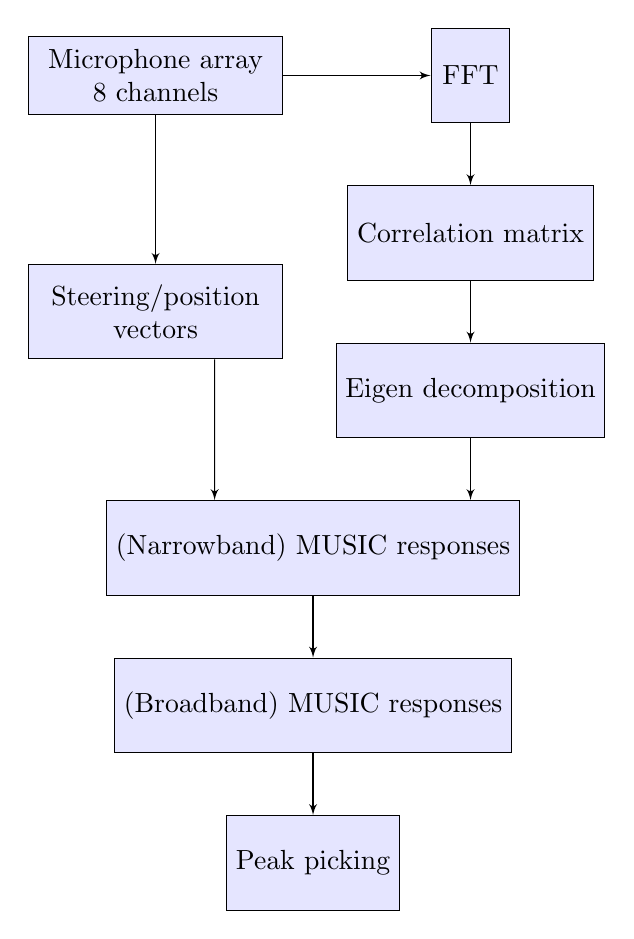
\begin{tikzpicture}[auto,node distance = 2 cm,>=latex', amp/.style = {regular polygon, regular polygon sides=3,
              draw, fill=white, text width=1em,
              inner sep=0.5mm, outer sep=0mm,
              shape border rotate=-90}
                        ]]
    % We start by placing the blocks
    \node [block, name=micro, minimum width=3cm, minimum height=1cm, text centered, text width=3cm] {Microphone array \\ 8 channels};
	\node [block, right of=micro, xshift=2cm] (fft) {FFT};    
    \node [block, below of=fft] (corr) {Correlation matrix};
    \node [block, below of=corr] (eig) {Eigen decomposition};
    \node [block,  below of=micro, yshift=-1cm, text centered, text width=3cm] (stee) {Steering/position \\ vectors};
    \node [block, below of=eig, xshift=-2cm] (mus) {(Narrowband) MUSIC responses};
    \node [block, below of=mus] (mus2) {(Broadband) MUSIC responses};
    \node [block, below of=mus2] (peak) {Peak picking};
    %\node [block,minimum height=2.2cm, minimum width=1.5cm, right of=zoh, xshift=1cm] (sat) {};
          
	% We draw an edge between the controller and system block to 
    % calculate the coordinate u. We need it to place the measurement block. 
      
    % Once the nodes are placed, connecting them is easy. 
    \draw [->] (micro) -- node[xshift=-0.5cm] {} (fft);
    \draw [->] (fft) -- node {} (corr);
    \draw [->] (corr) -- node[xshift=-1cm] {} (eig);
    \draw [->] (micro) -- node {} (stee);
    \draw [->] ([xshift=0.75cm]stee.south) -- node {} ([xshift=-1.25cm]mus.north);
    \draw [->] (eig) -- node {} ([xshift=2cm]mus.north);
    \draw [->] (mus) -- node {} (mus2);
    \draw [->] (mus2) -- node {} (peak);
     
   
\end{tikzpicture}
\caption{Block diagram of the sound source localization}
\label{fig:MUSICdiagram}
\end{figure}
\subsection{MUSIC algorithm}
\label{sec:MUSIC}
The Multiple Signal Classification algorithm can be defined as the determination of different parameters of multiple wavefronts that enter an array of antennas or sensors \cite{MUSIC}.
\\
The MUSIC algorithm provides asymptotically unbiased estimates of different parameters such as number of signals, direction of arrival (DOA), polarization, strength and cross correlation among the directional waveforms, and many others.
\newline
The $M$ array elements receive the waveforms from the sources that are linear combinations of the $D$ incidents wavefronts\footnote{explicar que es wavefront} and noise. This can be expressed as in equation \ref{equ:Xrec}.
%\begin{equation}

\begin{gather}
\label{equ:Xrec}
\begin{bmatrix}
X_1 \\ X_2 \\ \vdots \\ X_M
\end{bmatrix} = \begin{bmatrix}
\mathbf{a}(\theta_1) & \mathbf{a}(\theta_2) & \hdots & \mathbf{a}(\theta_D)
\end{bmatrix}
\begin{bmatrix}
F_1 \\ F_2 \\ \vdots \\ F_D
\end{bmatrix} + 
\begin{bmatrix}
W_1 \\ W_2 \\ \vdots \\ W_M
\end{bmatrix}  \\
 \text{or } \mathbf{X}  = \mathbf{A}\mathbf{F}+\mathbf{W} 
\end{gather}
%\end{equation}
where the vector $\mathbf{X}$ represents the $M$ received waveforms, the incident signals are represented by the vector $\mathbf{F}$ in phase and amplitude at some reference point, and the complex noise is represented by the vector $\mathbf{W}$. \\ The elements $a_{ij}$ from the matrix $\mathbf{A}$ are functions of the angle of arrival and the position of the array elements. Therefore, each element $a_{ij}$ depends on the position relative to the origin of the $ith$ array element and the response of the incident signal from the direction $jth$. The $jth$ column of matrix $\mathbf{A}$ is known as the mode vector of responses to the direction of arrival $\theta_j$ of the $jth$ signal. That is, the mode vector $\mathbf{a}_j$ is equivalently to the direction of arrival $\theta_j$.
\newline

It can be deducted from equation \ref{equ:Xrec} that the vector $\mathbf{X}$ is a linear combination of the mode vectors $\mathbf{a}(\theta_j)$ in which the elements of the matrix $\mathbf{F}$ are the coefficients of this combination. The directions of arrival of multiple incident wavefronts are calculated by determining the intersections of the $\mathbf{a}(\theta)$ continuum with the range space of $\mathbf{A}$.
\\
\newline
For determining the source localization, the correlation matrix of the input signals needs to be calculated. That is, the covariance matrix of the $\mathbf{X}$ vector is
\begin{equation}
\label{cov}
\mathbf{S}=\mathbf{X}\mathbf{X}^*=\mathbf{A}\mathbf{F}\mathbf{F}^*\mathbf{A}^*+\mathbf{W}\mathbf{W}^*.
\end{equation}
Where the * operator indicates the conjugate transpose operator. With the covariance matrix of the microphone array observations is performed a principal component analysis on this matrix to separate the disjoint signal and noise subspaces.
For these means, the eigenvalue decomposition or singular decomposition of the covariance matrix $\mathbf{S}$ is carried out. The M-th space correlation matrix obtained in \ref{cov} is decomposed in the signal and noise subspaces as per
\begin{equation}
\label{decomposition}
\mathbf{S}=\mathbf{Q}\mathbf{\Lambda}\mathbf{Q}^{-1}
\end{equation}
in which $\mathbf{Q}$ is a $M \times M$ matrix with the eigenvectors $\mathbf{q}_i$ of $\mathbf{S}$ written in the column i-th, and the matrix $\mathbf{\Lambda}$ is a diagonal matrix containing the eigenvalues. \\
The singular vectors $\mathbf{q}_i$ are orthogonal to the space spanned by the columns of $\mathbf{A}$ or in other words the vectors contained in the columns of $\mathbf{A}$ are perpendicular to each other. 
Since the eigenvectors $\mathbf{q}_i$ have correlation to the power of the incident wavefronts, the eigen vectors can be divided into $N$ noise eigenvectors and $D$ incident signal mode vectors, in which the $D$ vectors correspond to the eigenvalues with greatest value. For instance, the matrix $\mathbf{Q}$ can be written as
\begin{equation*}
\mathbf{Q}=[\mathbf{q}_1,\mathbf{q}_2,\hdots,\mathbf{q}_M]
\end{equation*}
and the split matrix gives the mode vectors \([\mathbf{q}_1,\mathbf{q}_2,\hdots,\mathbf{q}_D]\) and the noise eigenvectors \([\mathbf{q}_{1},\hdots,\mathbf{q}_{N}]\).
\newline

The next step is to solve for the incident mode vectors. In order to do that the spectrum for SSL is calculated using the noise eigenvectors as per
\begin{equation}
\label{spectrum}
P=\frac{\mid \mathbf{H}^* \mathbf{H}\mid}{\sum\limits_{i=1}^{N} \mid \mathbf{H}^*\mathbf{q}_{i} \mid}.
\end{equation} 
Where $\mathbf{H}$ is the transfer function of the sound propagation. The transfer function can be determined numerically or by measurements. The transfer function is a multichannel expression that depends on the sound $S_i$ in direction $\theta_i$ in view of the microphone array to the i-th microphone and is expressed as
\begin{equation}
\mathbf{H}=[H_1,\hdots,H_M].
\end{equation}
The transfer function is to be determined with anteriority and is also called as the steering vector.
\\
\newline
The numerator of equation \ref{spectrum} represents the multiplication between the steering vector (transfer function) and the noise-related eigenvector. This product is theoretically zero if the transfer function is a vector corresponding to the desired sound; making the quotient of the spectrum diverge infinitely. In reality, the denominator does not go exactly to zero due to the effects of noise but an abrupt peak can be observed.
\\ Equation \ref{spectrum} represents the spectrum for every frequency a broadband SSL is performed for the desired frequencies as
\begin{equation}
\hat{P}=\sum\limits_{\omega=\omega_{min}}^{\omega_{max}}W_{\Lambda}W_{\omega}P.
\end{equation}
$\omega_{min}$ and $\omega_{max}$ determine the desired frequency bands, $W_{\Lambda}$ is the eigenvalue weight and is the square root of the maximum eigenvalue. Finally, $W_{\\omega}$ is the spectrum weight factor. \\
\newline
The search of the sound is performed in the frequency bands aforementioned for $\hat{P}$ where the maxima are identified by local maximum searching or the hill-climbing method

\subsection{Sound source tracking}
Subsubsection text.

\subsection{Sound source separation}
Subsubsection text.

\subsection{Sound source recognition}
Subsubsection text.

\section{Experiment and result}

\subsection{Results}

\section{Zusammenfassung}
\label{sec:zus}


\appendices
\section{Optionaler Titel}
Anhang eins.
\section{}
Anhang zwei.



\section*{Danksagung}
Wenn ihr jemanden danken wollt, der Euch bei der Arbeit besonders
unterst�tzt hat (Korrekturlesen, fachliche Hinweise,...), dann ist hier der daf�r vorgesehene Platz.

\begin{thebibliography}{1}
\bibitem{IEEEhowto:kopka}
H.~Kopka and P.~W. Daly, \emph{A Guide to {\LaTeX}}, 3rd~ed. Harlow, England: Addison-Wesley, 1999.
\bibitem{wissPraxis:DFG}
Deutsche Forschungsgemeinschaft, \emph{Vorschl�ge zur Sicherung guter wissenschaftlicher Praxis}, Denkschrift, Weinheim: Wiley-VCH, 1998.

\bibitem{durkovic}
M. Durkovic: \emph{Localization, Tracking, and Separation of Sound Sources for Cognitive Robots}, PhD thesis, Technische Universi/"at M/"unchen (2012). 
  %(https://mediatum.ub.tum.de/1096033)
\bibitem{valin}
J.-M. Valin , F. Michaud , J. Rouat , D. Letourneau, \emph{Robust sound source localization using a microphone array on a mobile robot}, DOI: 10.1109/IROS.2003.1248813,  Proceedings 2003 IEEE/RSJ International Conference on Intelligent Robots and Systems (IROS 2003).  
%https://ieeexplore.ieee.org/document/1248813/
\bibitem{valin2}
J.-M. Valin, F. Michaud, J. Rouat, \emph{Robust Localization and Tracking of Simultaneous Moving Sound Sources Using Beamforming and Particle Filtering}, DOI: 10.1016/j.robot.2006.08.004, Robotics and Autonomous Systems Journal 55(3), 216-228 (2007).
%https://arxiv.org/abs/1602.08139
\bibitem{liu}
J. Liu, H. Erwin, S. Wermter, M. Elsaid, \emph{A Biologically Inspired Spiking Neural Network for Sound Localisation by the Inferior Colliculus}, Artificial Neural Networks - ICANN, Springer Berlin Heidelberg (2008).
% https://link.springer.com/chapter/10.1007/978-3-540-87559-8_41
\bibitem{murray}
J. C. Murray, H. Erwin, S. Wermter, \emph{A Hybrid Architecture Using Cross-Correlation and Recurrent Neural Networks for Acoustic Tracking in Robots}, Biomimetic Neural Learning for Intelligent Robots, Lecture Notes in Computer Science, vol 3575, Springer Berlin Heidelberg (2005).
% https://link.springer.com/chapter/10.1007/11521082_5

\bibitem{murase}
M. Murase, S. Yamamoto, J.-M. Valin, K. Nakadai, K. Yamada, K. Komatani?, T. Ogata, H. G. Okuno, \emph{Multiple Moving Speaker Tracking by Microphone Array on Mobile Robot}, Interspeech (2015).
% https://www.isca-speech.org/archive/archive_papers/interspeech_2005/i05_0249.pdf 
\bibitem{fazenda}
B. Fazenda, H. Atmoko, F. Gu, L. Guan, A. Ball: Acoustic based safety emergency vehicle detection for intelligent transport systems, ICCAS-SICE (2009).  
%https://ieeexplore.ieee.org/document/5332788/

\bibitem{shen}
G. Shen, Q. Nguyen, J. Choi, \emph{An Environmental Sound Source Classification System Based on Mel-Frequency Cepstral Coefficients and Gaussian Mixture Models}, IFAC proceedings, volume 45, Issue 6, pages 1802-1807 (2012).
%https://www.sciencedirect.com/science/article/pii/S1474667016334127

\bibitem{piczak}
K. J. Piczak, \emph{Environmental sound classification with convolutional neural networks}, DOI: 10.1109/MLSP.2015.7324337, IEEE 25th International Workshop on Machine Learning for Signal Processing (MLSP)  (2015). 
% https://ieeexplore.ieee.org/abstract/document/7324337/
\bibitem{baelde}
M. Baelde, C. Biernacki, R. Greff, \emph{A mixture model-based real-time audio sources classification method}, IEEE International Conference on Acoustics, Speech and Signal Processing (ICASSP)  (2017).
% https://ieeexplore.ieee.org/document/7952592
\end{thebibliography}
\end{document}\grid
\grid
